\documentclass[a4paper,notitlepage]{article}

\usepackage{xltxtra}
\usepackage{amsmath}
\usepackage{amssymb}
\usepackage{amsthm}
\usepackage{tikz}
\usetikzlibrary{shapes,arrows}
\usetikzlibrary{positioning}
\usepackage{unicode-math}
\usepackage{fontspec}
\usepackage[tikz]{dot2texi}
\setmathfont{xits-math.otf}
\usepackage{multicol}

\newtheorem{observation}{Observation}
\newtheorem{proposition}{Proposition}

\tikzset{node distance=2cm, auto}

\author{Víctor López Juan}
\title{Chapter 6}

\begin{document}

\maketitle

\begin{enumerate}
     
   \item[ 2.]

     \begin{enumerate}

       \item[a)]

         \begin{proposition}
           
         $$(A \times B)^C \cong A^C \times B^C$$

         \end{proposition}

         \begin{proof}

           We will prove that $(A^C \times B^C)$ {\em is} an exponential
           object $(A \times B)^C$. The isomorphism follows from the
           universality of exponentials.

           \begin{description}
             
             \item[Existence]
               
               Existence follows from the construction in this
               diagram, where $f : D \times C → A \times B$, and
               $\bar{f}$ is the unique transpose requiered by the definition
               of exponential object.

               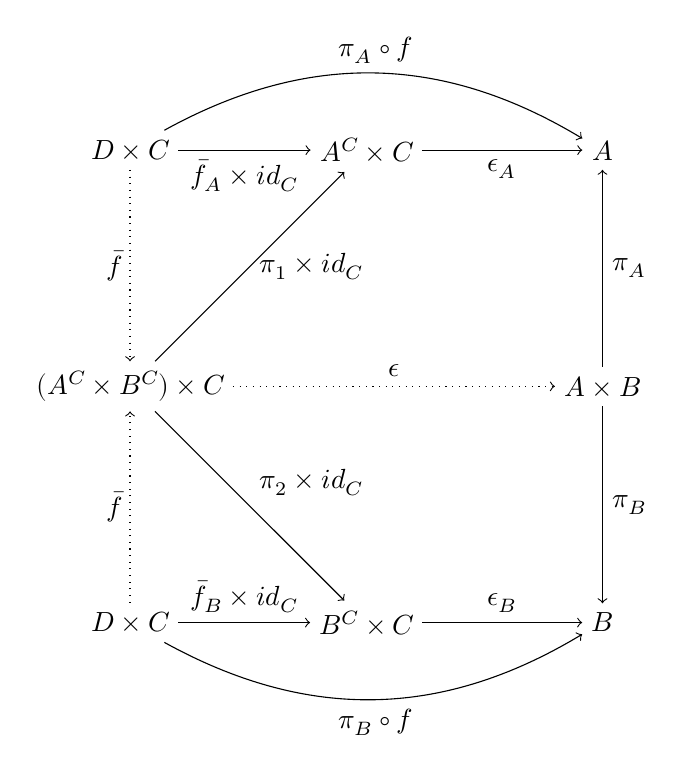
\begin{tikzpicture}[node distance=3cm]

                  \node (AcBc) {$(A^C \times B^C) \times C$};
                  

                  \node (DxC1) [above of=AcBc] {$D \times C$};
                  \node (DxC2) [below of=AcBc] {$D \times C$};

                  \node (Ac) [right of=DxC1] {$A^C \times C$};
                  \node (Bc) [right of=DxC2] {$B^C \times C$};

                  \node (A) [right of=Ac] {$A$};
                  \node (B) [right of=Bc] {$B$};

                  \node (AxB) [below of=A] {$A\times B$};

                  \draw [->] (AxB) to node[right] {$\pi_A$} (A);
                  \draw [->] (AxB) to node {$\pi_B$} (B);

                  \draw [->,bend left] (DxC1) to node {$\pi_A \circ f$} (A);   
                  \draw [->,bend right] (DxC2) to node[below] {$\pi_B \circ f$} (B);   

                  \draw [->,dotted] (AcBc) to node {$\epsilon$} (AxB);

                  \draw [->] (Ac) to node[below] {$\epsilon_A$} (A);
                  \draw [->] (Bc) to node {$\epsilon_B$} (B);

                  \draw [->] (DxC1) to node[below] {$\bar{f}_A \times id_C$} (Ac);
                  \draw [->] (DxC2) to node {$\bar{f}_B \times id_C$} (Bc);

                  \draw [->,dotted] (DxC1) to node[left] {$\bar{f}$} (AcBc);
                  \draw [->,dotted] (DxC2) to node {$\bar{f}$} (AcBc);

                  \draw [->] (AcBc) to node[right] {$\pi_1 \times id_C$} (Ac);
                  \draw [->] (AcBc) to node {$\pi_2 \times id_C$} (Bc);
             \end{tikzpicture}

               $\bar{f}_A$ and $\bar{f}_B$ are the transposes of
               $\pi_A \circ f$ and $\pi_B \circ f$ through $A^C$ and $B^C$,
               respectively.

               $\bar{f} \times id_C = \langle \bar{f}_A , \bar{f}_B \rangle \times id_C$,
               and $\epsilon = \langle \epsilon_A \circ (\pi_1 \times id_C), \epsilon_B \circ (\pi_2 \times id_C) \rangle$.

           \item[Uniqueness]

             Assume that there exists $z, {z^\prime} : D → (A^C \times B^C)$ such that
             
             $$f = \epsilon \circ z \times id_C = \epsilon \circ z^\prime \times id_C$$
             
             By the definition of product, 

             $$z = \langle z_A , z_B \rangle$$
             
             $$z^\prime = \langle z_A^\prime , z_B^\prime \rangle$$
             
             for $(\pi_A \circ z) = z_A : D → A^C$, $(\pi_B \circ z) = z_B : D → B^C$, and
             for $(\pi_A \circ z^\prime) = z_A^\prime : D → A^C$, $(\pi_B \circ z^\prime) = z_B^\prime : D → B^C$.

             Then:

             $$\pi_A \circ f = \epsilon_A \circ (\pi_1 \times id_C) \circ (z \times id_C) = \epsilon_A \circ (\pi_1 \times id_C) \circ (z^\prime \times id_C)$$

             $$\pi_A \circ f = \epsilon_A \circ (z_A \times id_C) = \epsilon_A \circ (z_A^\prime \times id_C)$$

             by the universality of $A^C$,

             $z_A = z_A^\prime$.

             Analogously for $z_B$:

             $$\pi_B \circ f = \epsilon_B \circ (\pi_2 \times id_C) \circ (z \times id_C) = \epsilon_B \circ (\pi_2 \times id_C) \circ (z^\prime \times id_C)$$

             $$\pi_B \circ f = \epsilon_B \circ (z_B \times id_C) = \epsilon_B \circ (z_B^\prime \times id_C)$$

             by the universality of $B^C$,

             $z_B = z_B^\prime$.

             Finally, by the universality of the product,

             $$z = \langle z_A, z_B \rangle = \langle z_A^\prime , z_B^\prime \rangle = z^\prime$$
             
         \end{description}
             
       \end{proof}

    \item[b)]

      \begin{proposition}
      $$(A^B)^C \cong A^{B \times C}$$

      \end{proposition}

      \begin{proof}
      We will prove that $(A^B)^C$ is an exponential object $A^{B \times C}$.
      The isomorphism follows because the exponential object is
      universal.

      \begin{description}

        \item[Existence] 


      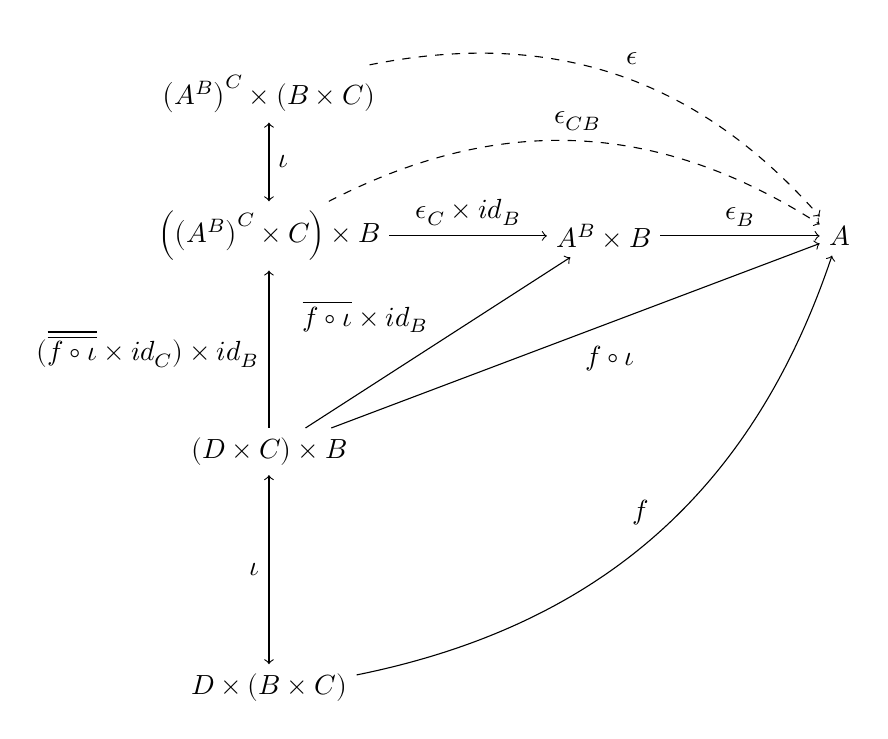
\begin{tikzpicture}[node distance=3cm]
        \node (ABC) {$\left (A^B \right )^C \times (B \times C)$};
        \node (ACB) [below=1 of ABC] {$\left ( \left ( A^B \right )^C \times C \right ) \times B$};
        \node (DCB) [below=2 of ACB] {$(D \times C) \times B$};
        \node (DBC) [below of= DCB] {$D \times (B \times C)$};
        
        \node (AB)  [right=2 of ACB] {$A^B \times B$};
        \node (A)   [right of=AB]  {$A$};

        \draw [->,bend right] (DBC) to node {$f$} (A);
        \draw [->,swap] (DCB) to node {$f \circ \iota$} (A);
        \draw [->] (DCB) to node {$\overline{f \circ \iota} \times id_B$} (AB);
        \draw [->] (DCB) to node {$(\overline{\overline{f \circ \iota}} \times id_C) \times id_B$} (ACB);

        \draw [<->] (ABC) to node {$\iota$} (ACB);
        \draw [<->] (DBC) to node {$\iota$} (DCB);

        \draw [->] (ACB) to node {$\epsilon_{C} \times id_B$} (AB);
        \draw [->] (AB) to node {$\epsilon_B$} (A);

        \draw [->, bend left, dashed] (ABC) to node {$\epsilon$} (A);
        
        \draw [->, bend left, dashed] (ACB) to node {$\epsilon_{CB}$} (A);

        %\draw [->,bend left] (DBC) to node {} (ABC);
      \end{tikzpicture}

      $\iota$ is the canonical isomorphism for the commutativity and
      associativity of products. 

      An overlined arrow name signifies the transpose of that function
      given some exponential object. The first overlining of $f \circ ι$ corresponds to the
      exponential object $A^B$, while the second one corresponds to
      $(A^B)^C$.

      Functors preserve commutativity of diagrams.
      In the case of $\left ( A^B \right )^C$, all the objects and arrows in the
      exponential object definition are mapped by the functor $(— \times B)$

      $$(— \times B)(X) = X \times B$$

      $$(— \times B)(α) = α \times id_B$$

      The transpose of $f$ together with the identity arrow is:

      \begin{equation*}
      \bar{f} \equiv \overline{\overline{f \circ \iota}} \times id_{B\times C} :
               D × (B × C) → \left (A^B \right )^C \times (B \times C)\text{ .}
      \end{equation*}
      
      The evaluation function $ε$ is constructed from the underlying
      exponential objects.

      $$\epsilon_{CB} \equiv \epsilon_B \circ (\epsilon_C × id_B)$$

      $$\epsilon \equiv ι  \epsilon_{CB}$$
      
      The diagram above commutes. 

      \item[Uniqueness]

        Let $z, z' : D  → (A^B)^C$, and
        $$z × id_{B \times C} , z^\prime × id_{B \times C}: D × (B × C) → (A^B)^C × (B × C)$$
        such that the diagram above commutes.

        The notation $\iota$ has been overloaded to stand for any of the
        two isomorphisms in the diagrams, in both directions. The
        specific arrow can be inferred from context.

        Then:

        $$f = \epsilon \circ \left ( z ×  id_{B \times C}  \right ) = \epsilon \circ \left ( z^\prime ×  id_{B \times C}  \right ) = f$$
        
        $$f \circ \iota = \epsilon \circ \left ( z ×  id_{B \times C}  \right ) \circ \iota = \epsilon \circ \left ( z^\prime ×  id_{B \times C}  \right ) \circ \iota = f \circ \iota$$
        
        $$f \circ \iota = \epsilon_{BC} \circ \iota \circ \left ( z ×  id_B × id_C  \right ) \circ \iota = \epsilon_{BC} \circ \iota \circ \left ( z^\prime ×  id_B × id_C  \right ) \circ \iota = f \circ \iota$$
        
        $$f \circ \iota = \epsilon_{BC} \circ \left ( \left ( z ×  id_C  \right ) ×   id_B  \right ) = \epsilon_{BC} \circ \left ( \left ( z^\prime ×  id_C  \right )  ×  id_B  \right )$$
        
        $$f \circ \iota = \epsilon_{B} \circ \left ( \epsilon_{C} ×  id_{B}  \right ) \circ \left ( \left ( z ×  id_C  \right ) ×  id_B  \right ) = \epsilon_{B} \circ \left ( \epsilon_{C} ×  id_B  \right ) \circ \left ( \left ( z^\prime ×  id_C  \right )  ×  id_B \right )$$
        
        $$f \circ \iota = \epsilon_{B} \circ \left ( \left ( \epsilon_C \circ \left ( z ×  id_C  \right ) \right ) × id_B \right )   = \epsilon_{B} \circ \left ( \left ( \epsilon_C \circ \left ( z^\prime ×  id_C  \right ) \right )  ×  id_B  \right )$$

        Universality of ($A^B$), $(— × B)$ is injective:
        $$\overline{f \circ \iota} = \epsilon_C \circ \left ( z × id_C \right ) = \epsilon_C \circ \left ( z^\prime × id_C \right )$$
        
        Universality of ($(A^B)^C$)
        $$z = z^\prime$$

     \end{description}

     \end{proof}

   \end{enumerate}

   \item[ 5.]

     $2^G$ is the set of functions $G → 2$.

     The exponential graph has $2^{\vert G \vert }$ vertices, one for each
     possible mapping from $G_v$ to $2_v = {v₁,v₂}$. Each mapping $\phi$ can be
     seen as a partition of the vertices in $G$ into two groups, $\phi^{-1}(v_1)$
     and $\phi^{-1}(v_2)$.

     According to the definition, for every pair of vertices $\phi$,
     $\psi : G_v → 2$, we define
     $\theta_{\phi,\psi} : G_e → 2_v \times 2_v$,
     $\theta_{\phi,\psi}(u,v) = (\phi(u), \psi(v))$.

     There is an edge $(\phi, \psi)$ in $2^G$ iff $\theta_{\phi,\psi}(G_e) \subseteq 2_e = {(v_1,v_2)}$.

     In this case, we can define two sets of vertices, $S = \{ u \vert (u,v) \in G_e \} \subseteq G_v$, and
     $T = \{ v \vert (u,v) \in G_e \} \subseteq G_V$.

     From this set, we define similar subsets in the exponential graph:

     $\bar{S} = \{ \phi \vert \phi \in G_v, \phi(S) \subseteq \{ v_1 \} \}$

     $\bar{T} = \{ \psi \vert \phi \in G_v, \psi(T) \subseteq \{ v_2 \} \}$

     The set of edges in the exponential graph is $S \times T$. In particular,
     every $\phi$ which is a graph homomorphism has a self-edge.

     {\em Example:} Construct the exponential graph $2^G$. 
     
     \begin{multicols}{2}
     
     \begin{dot2tex}[neato]
       \input{ex5.hs/graph2.dot}
     \end{dot2tex}
     
     \begin{dot2tex}[neato]
       \input{ex5.hs/graphG.dot}
     \end{dot2tex}

     \end{multicols}

     {\Large
     \begin{dot2tex}[fdp,autosize,scale=0.5]
       \input{ex5.hs/graph2toG.dot}
     \end{dot2tex}
     }
     
     The first graph is $2$, the second is $G$, and the last one is $2^G$.

     Notice the self-edge in node:

     $$ \left [ a \mapsto 1, b \mapsto 2, c \mapsto 1, d \mapsto 1 \right ] $$

     … which is a graph homomorphism itself.

     Haskell code is provided.

     
\end{enumerate}
\end{document}
  
